% ---------------------------------------------------------------------
\section{Giao thức và giao diện lập trình}\label{sec:giaothuc}
\begin{lstlisting}[language=json,caption={Bản tin \code{parking\_update} (Sensor Client → máy chủ)}]
{"type":"parking_update","slots":[1,0,0,1,0],"water_mm":0.2,"fire":false}
\end{lstlisting}
\begin{lstlisting}[language=json,caption={Bản tin \code{rfid\_event} (RFID Client → máy chủ)}]
{"type":"rfid_event","card_id":"A1B2C3D4","gate":"in","temperature_c":28.0}
\end{lstlisting}
\begin{lstlisting}[language=json,caption={Bản tin \code{climate} (RFID Client → máy chủ, mỗi 5\,s)}]
{"type":"climate","temperature_c":28.0}
\end{lstlisting}

\paragraph{Ký gói tin.} Mỗi bản tin JSON ở trên được gửi trong một ``phong bì'' có chữ ký;
máy chủ trả lời mỗi \code{rfid\_event} bằng một gói \code{ACK} cũng được ký:
\begin{lstlisting}[language={},numbers=none,caption={Định dạng gói UDP (\file{packet\_auth.c})}]
<tag: 16 hex><seq: 8 hex><JSON>         tag = SipHash-2-4(khoa 16 byte, seq + JSON)
16af4b44ee606cdf1234abcd{"type":"climate","temperature_c":28.0}
<tag><seq>ACK                           may chu -> RFID Client, cung seq voi su kien
\end{lstlisting}
\begin{itemize}[nosep]
  \item \textbf{Chữ ký} chứng minh gói đến từ thiết bị biết khóa: đổi bất kỳ byte nào
        (kể cả \code{seq}) thì chữ ký sai và gói bị bỏ trước khi đọc JSON.
  \item \textbf{Số thứ tự} \code{seq} chỉ tăng, kể cả qua lần khởi động lại của client
        (client giữ trước từng khối 65\,536 số trong EEPROM, mỗi khối chỉ ghi flash một
        lần). Máy chủ giữ một \textbf{cửa sổ chống phát lại} 32 số cho mỗi loại bản tin
        (giống IPsec): số mới được xử lý, số đã thấy là bản gửi lại (chỉ trả ACK), số
        cũ hơn cửa sổ là gói bị ghi lại để phát lại và bị bỏ.
\end{itemize}

\begin{lydo}[Tại sao SipHash-2-4 thay vì HMAC-SHA256]
SipHash là hàm băm có khóa (PRF) thiết kế riêng cho thông điệp ngắn: một gói của nhóm
chỉ 70–130 byte. Chữ ký 64 bit đủ chống giả mạo trong bối cảnh này (kẻ tấn công phải
gửi trung bình $2^{63}$ gói để đoán trúng). Thuật toán chỉ khoảng 30 dòng C, giống hệt
trên ESP32-C3, ESP8266 và Python, nên cả ba nơi dùng chung một định dạng và bộ kiểm thử
kiểm tra được bằng vector chuẩn của tác giả. HMAC-SHA256 có sẵn trong mbedTLS (máy chủ)
và BearSSL (ESP8266) nhưng hai thư viện có API khác nhau, phải mô phỏng thêm trong bộ
kiểm thử, và chữ ký dài gấp bốn.
\end{lydo}

\begin{table}[H]
\centering\small
\caption{Đặc tả trường dữ liệu và ràng buộc kiểm tra trên máy chủ}\label{tab:fields}
\begin{tabularx}{\linewidth}{@{}llX@{}}
\toprule
\textbf{Trường} & \textbf{Kiểu} & \textbf{Ràng buộc} \\ \midrule
\code{type} & chuỗi & \code{"parking\_update"}, \code{"rfid\_event"} hoặc \code{"climate"} \\
\code{slots} & mảng & Đúng 5 phần tử, mỗi phần tử 0 (trống) hoặc 1 (có xe) \\
\code{water\_mm} & số & $0 \le x \le 10\,000$ \\
\code{fire} & boolean & Tùy chọn (client cũ có thể không gửi); không chấp nhận 0/1 \\
\code{card\_id} & chuỗi & 1–31 ký tự \code{[A-Za-z0-9\_-]}, chuẩn hóa thành chữ hoa \\
\code{gate} & chuỗi & \code{"in"} hoặc \code{"out"} (không phân biệt hoa thường) \\
\code{temperature\_c} & số & $-40 \le x \le 125$ \\
Chung & — & Khóa lạ, khóa lặp, dữ liệu thừa sau \code{\}}, chuỗi có ký tự thoát đều bị từ chối \\
\bottomrule
\end{tabularx}
\end{table}

\begin{table}[H]
\centering\small
\caption[API HTTP của máy chủ (12 route)]{API HTTP của máy chủ (12 route); mọi lệnh POST cần header \code{X-Parking-Key} đúng mã PIN, sai thì trả 401}\label{tab:api}
\begin{tabularx}{\linewidth}{@{}lp{4.4cm}X@{}}
\toprule
\textbf{PT} & \textbf{Đường dẫn} & \textbf{Kết quả} \\ \midrule
GET & \code{/}, \code{/style.css} & Trang web nhúng trong firmware \\
GET & \code{/api/parking} & \code{received}, \code{slots}, \code{free}, \code{total}, \code{temperature\_c}, \code{water\_mm}, \code{fire} \\
GET & \code{/api/barrier} & \code{\{"in\_open":bool,"out\_open":bool\}} \\
GET & \code{/api/rfid} & \code{now\_s}, \code{fee\_per\_hour}, \code{parked[]} (thẻ, giờ vào, phí tạm tính), \code{log[]} (10 sự kiện mới nhất) \\
POST & \code{/api/barrier/}\allowbreak\code{<cổng>/<lệnh>} & Cổng \code{in}, \code{out}, \code{all}; lệnh \code{open}, \code{close}. Lỗi 500 nếu bị từ chối (ví dụ đóng khi có cháy) \\
POST & \code{/api/time} & Thân là giờ Unix (giây) từ trình duyệt; máy chủ đặt đồng hồ bãi và lưu NVS \\
\bottomrule
\end{tabularx}
\end{table}

% ---------------------------------------------------------------------
\section{Thiết kế chi tiết từng thành phần}\label{sec:chitiet}

\subsection{Thanh chắn: PWM phần cứng và hẹn giờ một lần}
Servo SG90 nhận xung chu kỳ 20\,ms; độ rộng xung quyết định góc (Hình~\ref{fig:pwm}).
\begin{figure}[H]
\centering
\begin{tikzpicture}[x=0.55cm,y=0.7cm,font=\scriptsize]
\draw[-{Stealth}] (0,0) -- (23,0) node[right]{$t$ (ms)};
\draw[-{Stealth}] (0,0) -- (0,1.8) node[left]{PWM};
\draw[thick,accent] (0,0) -- (0,1.2) -- (1.45,1.2) -- (1.45,0) -- (20,0) -- (20,1.2) -- (21.45,1.2) -- (21.45,0) -- (22.5,0);
\draw[{Stealth}-{Stealth}] (0,-0.5) -- node[below]{chu kỳ $T = 20$\,ms (50\,Hz)} (20,-0.5);
\draw[{Stealth}-{Stealth}] (0,1.5) -- node[above]{$p$} (1.45,1.5);
\node[align=left,anchor=west] at (3,1.0) {$p = 500$\,µs $\to 0°$\quad $p = 1450$\,µs $\to 90°$\quad $p = 2400$\,µs $\to 180°$};
\end{tikzpicture}
\caption{Dạng xung điều khiển servo SG90}\label{fig:pwm}
\end{figure}
\begin{equation}
  p(\theta) = 500 + \frac{1900\,\theta}{180}\ \text{µs}, \qquad
  D = \left\lfloor \frac{p \cdot (2^{14}-1)}{20\,000} \right\rfloor
\end{equation}
Với $\theta=90°$: $p=1450$\,µs, $D=1187$; với $\theta=0°$: $p=500$\,µs, $D=409$.

\begin{lydo}[Tại sao 50\,Hz, 14 bit, LEDC]
\textbf{50\,Hz} là tần số chuẩn của servo RC analog. \textbf{14 bit} là độ phân giải
lớn nhất của LEDC trên ESP32-C3: mỗi bước $20\,000/16\,384 \approx 1{,}22$\,µs $\approx 0{,}12°$,
mịn hơn nhiều vùng chết $\approx$1° của SG90 nên servo không rung. \textbf{LEDC} là PWM
phần cứng: xung phát liên tục mà CPU không can thiệp, servo giữ góc ổn định dù
Wi-Fi hay màn hình đang bận. Dải 500–2400\,µs là giá trị đo thực tế của SG90 (danh
nghĩa 1000–2000\,µs không đủ 180°).
\end{lydo}

\begin{lydo}[Tại sao dùng hẹn giờ một lần (\code{esp\_timer}) thay vì tác vụ hỏi vòng]
Phiên bản đầu dùng một tác vụ thức dậy 20 lần/giây để kiểm tra hạn đóng. Phiên bản
hiện tại tạo một \code{esp\_timer} một lần cho mỗi cổng: hàm đóng được gọi \emph{đúng}
lúc hết 3\,s (sai số micro giây thay vì 50\,ms), CPU không bị đánh thức vô ích và tiết
kiệm 3\,KB stack. Vì một lệnh khác có thể ``đua'' với hàm đóng, hàm đóng kiểm tra lại
hạn đóng dưới mutex; lệnh tay từ web đặt hạn về 0 và dừng hẹn giờ — \textbf{lệnh của
người vận hành luôn thắng}.
\end{lydo}

Hai cổng được mô tả bằng cùng một cấu trúc (kênh LEDC, chân, hướng lắp, trạng thái,
hạn đóng, hẹn giờ) nên một hàm xử lý cho cả hai. Thanh chắn ra lắp đối xứng nên góc
mở/đóng đảo ngược (0° mở, 90° đóng) — chỉ khai báo ở một hàm. Cả hai cổng \textbf{luôn
khởi động ở vị trí đóng}, nên trạng thái không cần lưu vào flash; phiên bản trước ghi
NVS mỗi lần thanh chắn chuyển động đã được bỏ (chậm và làm mòn flash vô ích).

\subsection{Màn hình: SPI DMA, vẽ theo sự kiện, ảnh động tiền xử lý}
\begin{lydo}[Tại sao SPI 40\,MHz và DMA]
Một khung hình đầy đủ là $240\times240\times16 = 921\,600$ bit; ở 40\,MHz mất
$\approx$ 23\,ms, tối đa $\approx$ 43 khung/giây — dư cho giao diện tĩnh và màn hình cháy
8 khung/giây. 40\,MHz bằng đúng $80\,\text{MHz}/2$ (không sai số chia tần) và dưới giới
hạn ghi $\approx$ 62\,MHz của ST7789, chừa biên an toàn cho dây cắm. DMA cho phép CPU
làm việc khác trong lúc ảnh được đẩy ra.
\end{lydo}

\begin{itemize}
\item \textbf{Framebuffer RGB565} 115\,200 byte: toàn bộ giao diện được vẽ vào RAM rồi gửi
  một lần. Màu được lưu sẵn theo thứ tự byte của ST7789 (byte cao trước) vì
  ESP32-C3 là little-endian.
\item \textbf{Hàm tô hình chữ nhật} cắt biên một lần và tô từng dòng liên tục thay vì
  kiểm tra biên và đảo byte cho từng điểm ảnh.
\item \textbf{Font 5$\times$7 tự định nghĩa} cho A–Z, 0–9 (180 byte) — không cần thư viện
  đồ họa lớn như LVGL cho một giao diện cố định.
\item \textbf{Vẽ theo sự kiện}: \file{udp\_server} đánh thức tác vụ màn hình bằng thông
  báo tác vụ ngay khi có dữ liệu; nếu không có gì, tác vụ chỉ thức mỗi 1\,s (để hết hạn
  hóa đơn/thông báo) hoặc 120\,ms khi có cháy (để lửa nhấp nháy). Màn hình chỉ vẽ lại
  khi nội dung thực sự thay đổi.
\end{itemize}

\begin{table}[H]
\centering\small
\caption{Dữ liệu ảnh động sau tiền xử lý và nén LZSS}\label{tab:lzss}
\begin{tabular}{@{}lrrrr@{}}
\toprule
\textbf{Ảnh} & \textbf{Kích thước} & \textbf{Số khung} & \textbf{Dữ liệu thô} & \textbf{Sau nén} \\ \midrule
Kaoruko & 96$\times$96 & 10 & 184\,320 B & 70\,564 B (2,6$\times$) \\
Claude & 68$\times$46 & 18 & 112\,608 B & 16\,204 B (6,9$\times$) \\
\bottomrule
\end{tabular}
\end{table}

\begin{lydo}[Tại sao tiền xử lý ảnh trên máy tính]
Ảnh gốc có nền trắng cần xóa và điểm ảnh cần đảo byte. Phiên bản trước làm việc
này trên chip cho \emph{mọi khung hình}, 10 lần/giây: thuật toán loang tìm nền trắng
nối với viền (cần thêm 1,2\,KB RAM) rồi đảo byte 9\,216 điểm. Vì ảnh không bao giờ
đổi, nhóm làm một lần trên máy tính và lưu kết quả đã xử lý: firmware chỉ còn giải
nén. Kết quả được kiểm chứng giống từng điểm ảnh với cách cũ trên cả 28 khung, dữ
liệu còn nhỏ hơn (86\,768 so với 87\,977 byte). LZSS có bộ giải nén $\approx$ 40 dòng,
không cần bộ nhớ phụ và kiểm tra biên đầy đủ nên dữ liệu hỏng không gây ghi tràn.
\end{lydo}

\textbf{Hai bộ đệm DMA} (2 $\times$ 18\,432 byte) được dùng luân phiên cho ảnh động:
lệnh vẽ chỉ \emph{xếp hàng} giao dịch DMA rồi trả về, nên giải nén khung kế tiếp vào
cùng bộ đệm khi DMA chưa đọc xong sẽ làm hình bị xé. Hai tác vụ cùng vẽ lên một
panel nên dùng chung một mutex.

\subsection{Bộ kiểm tra bản tin JSON}
\begin{lydo}[Tại sao tự viết thay vì dùng thư viện cJSON]
Gói UDP là \emph{ranh giới tin cậy}: bất kỳ thiết bị nào trong mạng đều gửi được.
cJSON cấp phát heap cho từng nút (phân mảnh heap khi chạy lâu) và chấp nhận mọi JSON
hợp lệ. Bộ đọc tự viết (\file{json\_scan.c}, 81 dòng, dùng chung cho cả hai loại bản
tin) \textbf{không cấp phát động}, chỉ chấp nhận đúng lược đồ (Bảng~\ref{tab:fields})
và có \textbf{vòng lặp giới hạn} (tối đa 4 khóa) nên thời gian xử lý bị chặn trên.
Bộ đệm nhận 256 byte, đọc tối đa 255 byte và luôn kết thúc bằng \code{'\textbackslash0'}.
\end{lydo}

\subsection{Phiên gửi xe, phí, thông báo và nhật ký}
\begin{itemize}
\item \textbf{Phiên}: mảng tĩnh 5 phần tử — bằng số chỗ đỗ, không có nhiều xe hơn số chỗ.
  Thời điểm vào lấy từ \code{esp\_timer\_get\_time()} (64 bit, micro giây, không tràn trong
  hơn 290\,000 năm).
\item \textbf{Phí}: $h=\max(1,\lceil t/3600\rceil)$, phí $=5000\,h$ VNĐ, tính bằng số
  nguyên \code{(t + 3599) / 3600}, bão hòa ở \code{UINT32\_MAX} nếu tràn.
\item \textbf{Thông báo từ chối} (sai cổng, bãi đầy): giữ 5\,s; lần quẹt hợp lệ tiếp
  theo xóa thông báo ngay.
\item \textbf{Nhật ký}: bộ đệm vòng 10 sự kiện ($\approx$ 520 byte), đọc ra theo thứ tự mới
  nhất trước; không dùng heap.
\end{itemize}

\begin{lydo}[Tại sao chọn các thông số này]
\textbf{5.000\,VNĐ/giờ, làm tròn lên, tối thiểu 1 giờ} là cách tính phổ biến của bãi
xe, dễ giải thích. \textbf{Hóa đơn 60\,s} đủ để tài xế đọc và trả tiền; \textbf{thông
báo 5\,s} đủ đọc mà không che hóa đơn quá lâu. \textbf{Thanh chắn mở 3\,s} đủ cho xe mô
hình đi qua nhưng không đủ để xe sau ``đi ké''. \textbf{Nhật ký 10 sự kiện} vừa một màn
hình điện thoại và tốn dưới 1\,KB RAM.
\end{lydo}

\subsection{Sensor Client: lọc nhiễu và gửi theo thay đổi}
\begin{figure}[H]
\centering
\begin{tikzpicture}[x=0.9cm,y=0.6cm,font=\scriptsize]
\node[anchor=east] at (-0.2,2.5) {Tín hiệu thô};
\draw[thick] (0,2) -- (2,2) -- (2,3) -- (2.3,3) -- (2.3,2) -- (2.5,2) -- (2.5,3) -- (2.7,3) -- (2.7,2) -- (2.9,2) -- (2.9,3) -- (11,3);
\node[anchor=east] at (-0.2,0.5) {Trạng thái};
\draw[thick,accent] (0,0) -- (3.9,0) -- (3.9,1) -- (11,1);
\draw[dashed,gray] (2.9,3.3) -- (2.9,-0.4);
\draw[dashed,gray] (3.9,3.3) -- (3.9,-0.4);
\draw[{Stealth}-{Stealth}] (2.9,-0.6) -- node[below]{ổn định 50\,ms} (3.9,-0.6);
\node[align=center] at (2.45,3.8) {nhiễu khi xe\\đang lăn vào};
\node[draw,fill=boxB,align=center] at (7.5,-0.9) {gửi \code{parking\_update} ngay};
\draw[-{Stealth},thick] (3.9,1) to[bend right=10] (6.2,-0.6);
\end{tikzpicture}
\caption{Chống rung: chỉ chấp nhận mức mới khi giữ ổn định 50\,ms, rồi gửi ngay}\label{fig:debounce}
\end{figure}

\begin{lydo}[Tại sao lọc 50\,ms và gửi theo thay đổi kèm nhắc lại 1\,s]
Mép xe và bánh xe làm tín hiệu IR bật/tắt liên tục trong vài chục mili giây khi xe
đang vào chỗ. Nhóm tinh chỉnh thực nghiệm từ 250\,ms xuống \textbf{50\,ms}: đủ lọc nhiễu
mà cảm giác tức thời. Trước đây trạng thái chỉ được gửi theo chu kỳ 1\,s nên thay đổi
có thể trễ đến 1\,s; nay \textbf{gửi ngay khi có thay đổi}, đồng thời vẫn \textbf{nhắc
lại mỗi giây} để một gói bị mất được sửa ở lần sau. Mỗi cảm biến có bộ đếm riêng.
\end{lydo}

Mực nước được quy đổi tuyến tính từ ADC 10 bit:
\begin{equation}
  h_{\text{mm}} =
  \begin{cases}
  0, & raw \le 20 \\[2pt]
  \dfrac{\min(raw, 700) - 20}{700 - 20} \cdot 40, & raw > 20
  \end{cases}
\end{equation}
trong đó 20 là mức nhiễu khi khô, 700 là giá trị khi ngập hoàn toàn và 40\,mm là
chiều dài vùng đo; ADC được đọc mỗi 250\,ms vì đọc quá dày ảnh hưởng Wi-Fi trên
ESP8266 trong khi mực nước thay đổi chậm.

\subsection{RFID Client: hai đầu đọc trên một bus SPI}
\begin{lydo}[Tại sao bật ăng-ten luân phiên, chờ 4\,ms, gain 48\,dB, chống lặp 2\,s]
Hai đầu đọc 13,56\,MHz đặt gần nhau sẽ \textbf{nhiễu chéo}; chỉ bật một ăng-ten tại
một thời điểm loại bỏ hoàn toàn vấn đề. Thẻ thụ động cần vài mili giây để nhận đủ năng
lượng: \textbf{4\,ms} đủ cho thẻ MIFARE mà chu kỳ quét vẫn ngắn. \textbf{Gain 48\,dB} bù
tầm đọc khi đầu đọc nằm sau vỏ mô hình. Thẻ để yên sẽ bị đọc liên tục; \textbf{chống
lặp 2\,s} áp dụng cho cả hai đầu đọc, tránh một lần quẹt bị gửi nhiều lần làm ``vào''
biến thành ``ra''. UID được đổi sang chuỗi hex bằng \textbf{bộ đệm cố định} thay vì
\code{String} của Arduino: không cấp phát heap mỗi lần quẹt, nên heap 80\,KB của
ESP8266 không bị phân mảnh khi chạy lâu. DHT11 đọc mỗi \textbf{5\,s} vì cảm biến cần ít
nhất 1\,s giữa hai lần đọc và nhiệt độ thay đổi chậm.
\end{lydo}

\subsection{Trang web}
\begin{lydo}[Tại sao hỏi vòng 1–2\,s thay vì WebSocket]
Hỏi vòng không giữ trạng thái kết nối trên máy chủ: mỗi request độc lập, xử lý xong
giải phóng ngay — phù hợp giới hạn socket và RAM, và đơn giản khi nhiều trình duyệt
cùng xem. Với dữ liệu thay đổi theo giây, độ trễ thêm tối đa 1\,s là chấp nhận được.
Trang web là HTML/CSS/JavaScript thuần, nhúng trong firmware bằng
\code{EMBED\_TXTFILES}: không cần phân vùng tệp, không phụ thuộc CDN (điện thoại kết nối
hotspot không có Internet).
\end{lydo}

% ---------------------------------------------------------------------
\section{Phân tích kiến trúc}\label{sec:phantich}
\subsection{Hiệu năng và độ trễ}
\begin{table}[H]
\centering\small
\caption{Ngân sách độ trễ của các luồng chính (ước tính từ thông số thiết kế)}\label{tab:latency}
\begin{tabularx}{\linewidth}{@{}lXr@{}}
\toprule
\textbf{Luồng} & \textbf{Thành phần} & \textbf{Tổng} \\ \midrule
Xe vào ô → màn hình TFT & lọc 50\,ms + gửi ngay + UDP vài ms + đánh thức + vẽ 23\,ms & $\approx$ 0,1\,s \\
Xe vào ô → trang web & như trên + hỏi vòng tối đa 1\,s & $\le$ 1,1\,s \\
Quẹt thẻ → thanh chắn mở & quét 2 đầu đọc $\approx$ 10\,ms + UDP + xử lý $<$ 1\,ms + servo 90° $\approx$ 0,15\,s & $\approx$ 0,2\,s \\
Có lửa → còi kêu & lọc 50\,ms + gửi ngay + UDP & $\approx$ 0,06\,s \\
Mất một gói \code{parking\_update} & sửa ở lần nhắc lại & $\le$ 1\,s \\
Mất một gói \code{rfid\_event} & gửi lại sau 300\,ms chờ ACK & $\approx$ 0,5\,s \\
\bottomrule
\end{tabularx}
\end{table}

\subsection{Bộ nhớ}
\begin{table}[H]
\centering\small
\caption{Sử dụng bộ nhớ của firmware máy chủ (đo bằng \code{idf.py size})}\label{tab:memory}
\begin{tabularx}{\linewidth}{@{}Xr@{}}
\toprule
\textbf{Hạng mục} & \textbf{Kích thước} \\ \midrule
DRAM tĩnh dùng / tổng (mã IRAM 81\,444 + \code{.data} 13\,792 + \code{.bss} 21\,504) & 116\,740 / 321\,296 B (36,3\%) \\
Framebuffer màn hình (heap, DMA) & 115\,200 B \\
2 bộ đệm ảnh động (heap, DMA) & 36\,864 B \\
Stack các tác vụ của ứng dụng & $\approx$ 19\,KB \\
Bảng phiên, hóa đơn, thông báo, nhật ký, cửa sổ chống phát lại & $<$ 1\,KB \\ \midrule
Ảnh firmware & 1\,092\,768 B \\
Phân vùng ứng dụng (\code{factory}) & 1\,536\,000 B (dùng 71,1\%) \\
\bottomrule
\end{tabularx}
\end{table}

\begin{lydo}[Tại sao phân vùng ứng dụng 1,5\,MB]
Bảng phân vùng mặc định chỉ có 1\,MB cho ứng dụng và đã đầy 98\% trước khi thêm mDNS.
Flash 2\,MB đủ chỗ cho phân vùng 1,5\,MB có sẵn trong ESP-IDF
(\code{partitions\_singleapp\_large.csv}), được khai báo trong \file{sdkconfig.defaults}
để mọi thành viên build ra cùng cấu hình; còn 29\% dự phòng cho tính năng mới.
\end{lydo}

\subsection{Độ tin cậy và khả năng chịu lỗi}
\begin{table}[H]
\centering\small
\caption{Phân tích lỗi và cách hệ thống phản ứng}\label{tab:faults}
\begin{tabularx}{\linewidth}{@{}p{4.3cm}X@{}}
\toprule
\textbf{Tình huống lỗi} & \textbf{Phản ứng của hệ thống} \\ \midrule
Mất gói UDP cảm biến & Bản tin nhắc lại sau $\le$ 1\,s sửa trạng thái \\
Mất gói quẹt thẻ hoặc gói ACK & RFID Client gửi lại mỗi 300\,ms (tối đa 6 lần); máy chủ nhận bản sao chỉ trả ACK, không mở cổng hai lần \\
Bản tin sai định dạng / độc hại & Bị từ chối, trạng thái cũ giữ nguyên, có cảnh báo trong log \\
Gói không có chữ ký, sai khóa hoặc phát lại & Bị bỏ trước khi đọc JSON \\
Xe vào không quẹt thẻ (đi theo xe trước) & Trang web cảnh báo lệch số thẻ / số ô có xe; khi IR báo đủ 5 ô thì từ chối thẻ mới \\
Socket UDP lỗi & Đóng socket, chờ 1\,s, tạo lại \\
Máy chủ mất Wi-Fi & Tự kết nối lại; nhận IP (có thể mới) → thông báo lại \code{parking.local} \\
Client mất Wi-Fi & Sensor Client bỏ qua lần gửi, tự kết nối lại; trang web báo OFFLINE \\
DHT11 đọc lỗi & Giữ giá trị hợp lệ gần nhất \\
Có cháy khi người vận hành bấm đóng & Lệnh đóng bị từ chối; thanh chắn giữ mở \\
Máy chủ mất điện, khởi động lại & Thanh chắn về vị trí đóng; phiên, nhật ký, cửa sổ chống phát lại và đồng hồ được khôi phục từ NVS; thời gian mất điện được bù khi trình duyệt gửi giờ thực \\
Lỗi khởi tạo phần cứng & Fail-fast: in lỗi và khởi động lại \\
\bottomrule
\end{tabularx}
\end{table}

\subsection{Bảo mật}
\begin{itemize}
\item \textbf{Đã có}: kiểm tra bản tin chặt chẽ ở ranh giới mạng; không cấp phát động
  khi xử lý dữ liệu ngoài; mã thẻ giới hạn ký tự nên không thể chèn mã vào JSON hay
  HTML; trang web chèn dữ liệu bằng \code{textContent}, không dùng \code{innerHTML}
  cho dữ liệu từ máy chủ; mạng dùng WPA2.
\item \textbf{Xác thực bản tin}: mọi gói UDP được ký bằng SipHash-2-4 với khóa 16 byte
  dùng chung; gói giả (thẻ giả, báo cháy giả) và gói ghi lại để phát lại đều bị bỏ.
  Biết mật khẩu Wi-Fi \emph{không} đủ để điều khiển hệ thống.
\item \textbf{Xác thực API}: mọi lệnh thay đổi trạng thái (mở/đóng cổng, đặt giờ) cần mã
  PIN quản trị; so sánh mã PIN không dừng sớm để không lộ qua thời gian phản hồi.
\item \textbf{Bí mật ngoài mã nguồn}: mật khẩu Wi-Fi, khóa và mã PIN nằm trong
  \file{sdkconfig} (menuconfig) và \file{secrets.h}, cả hai bị \file{.gitignore} bỏ qua;
  kho mã chỉ chứa giá trị demo.
\end{itemize}

\subsection{Khả năng bảo trì, kiểm thử và mở rộng}
\begin{itemize}
\item Lớp nghiệp vụ độc lập phần cứng: 318 phép kiểm thử chạy trên máy tính trong vài giây.
\item Hai client được kiểm thử bằng chính mã nguồn \file{.ino} trên phần cứng giả lập,
  kèm kiểm tra hợp đồng giao tiếp với bộ đọc JSON thật của máy chủ.
\item Số chỗ đỗ là hằng số \code{PARKING\_SLOT\_COUNT}; số phiên tối đa bằng số chỗ.
  Mở rộng quy mô lớn hơn cần đổi định dạng \code{slots} và tách cảm biến theo khu vực.
\end{itemize}

\subsection{Tổng hợp quyết định kiến trúc}
\begin{longtable}{@{}p{3.3cm}p{3.6cm}p{7.4cm}@{}}
\caption{Các quyết định kiến trúc chính}\label{tab:adr}\\
\toprule \textbf{Quyết định} & \textbf{Phương án khác} & \textbf{Lý do / đánh đổi} \\ \midrule \endfirsthead
\toprule \textbf{Quyết định} & \textbf{Phương án khác} & \textbf{Lý do / đánh đổi} \\ \midrule \endhead
3 bo mạch, máy chủ trung tâm & 1 bo lớn & Đủ chân, đặt cảm biến gần nơi cần đo, cô lập lỗi; đổi lại cần mạng \\
FreeRTOS trên máy chủ & Vòng lặp Arduino & Nhiều việc song song có ưu tiên; đổi lại phải đồng bộ cẩn thận \\
UDP broadcast + JSON & TCP, MQTT, nhị phân & Nhẹ, dễ gỡ lỗi; mất gói được bù bằng nhắc lại (cảm biến) hoặc ACK và gửi lại (quẹt thẻ) \\
Ký gói bằng SipHash + số thứ tự & HMAC-SHA256, TLS & Cùng một mã 30 dòng trên 3 nền tảng, kiểm thử được; chữ ký 64 bit \\
Gửi theo thay đổi + nhắc lại 1\,s & Chỉ gửi định kỳ & Độ trễ $\approx$ 0,1\,s; vẫn tự sửa khi mất gói \\
Điểm truy cập trên RFID Client + mDNS & AP trên máy chủ, router & Dành RAM máy chủ cho màn hình; tên cố định dù IP đổi \\
Bộ đọc JSON tự viết & cJSON & Không cấp phát, chỉ đúng lược đồ; đổi lại phải tự kiểm thử kỹ \\
Hẹn giờ một lần cho thanh chắn & Tác vụ hỏi vòng & Chính xác, không đánh thức CPU vô ích \\
Vẽ màn hình theo sự kiện & Hỏi vòng 500\,ms & Phản hồi ngay, ít lần thức \\
Tiền xử lý ảnh động trên máy tính & Xử lý trên chip mỗi khung & Bớt CPU và 1,2\,KB RAM; dữ liệu nhỏ hơn \\
Lưu phiên/nhật ký vào NVS sau mỗi lần quẹt và mỗi 5 phút & Chỉ giữ trong RAM; ghi mỗi giây & Không mất dữ liệu khi mất điện; NVS tự rải lượt ghi, $\approx$ 300 lần ghi/ngày là rất nhỏ so với tuổi thọ flash \\
Giờ thực do trình duyệt cung cấp & SNTP, RTC DS3231 & Mạng không có Internet nên SNTP không dùng được; không cần thêm phần cứng \\
\bottomrule
\end{longtable}

% ---------------------------------------------------------------------
\section{Demo}\label{sec:demo}
\subsection{Trang web giám sát}
Hình~\ref{fig:dashboard} là ảnh chụp trang web thật của hệ thống (chạy với dữ liệu mẫu).
Sơ đồ bãi là phần chính: 5 ô lớn, ô có xe vẽ hình xe màu đỏ, ô trống hiện chữ P màu
xanh, làn xe với hướng vào/ra; phía trên là số chỗ trống/có xe/tổng. Bên dưới là điều
khiển thanh chắn, cảm biến và nhật ký vào/ra kèm giá gửi xe.

\begin{figure}[H]
\centering
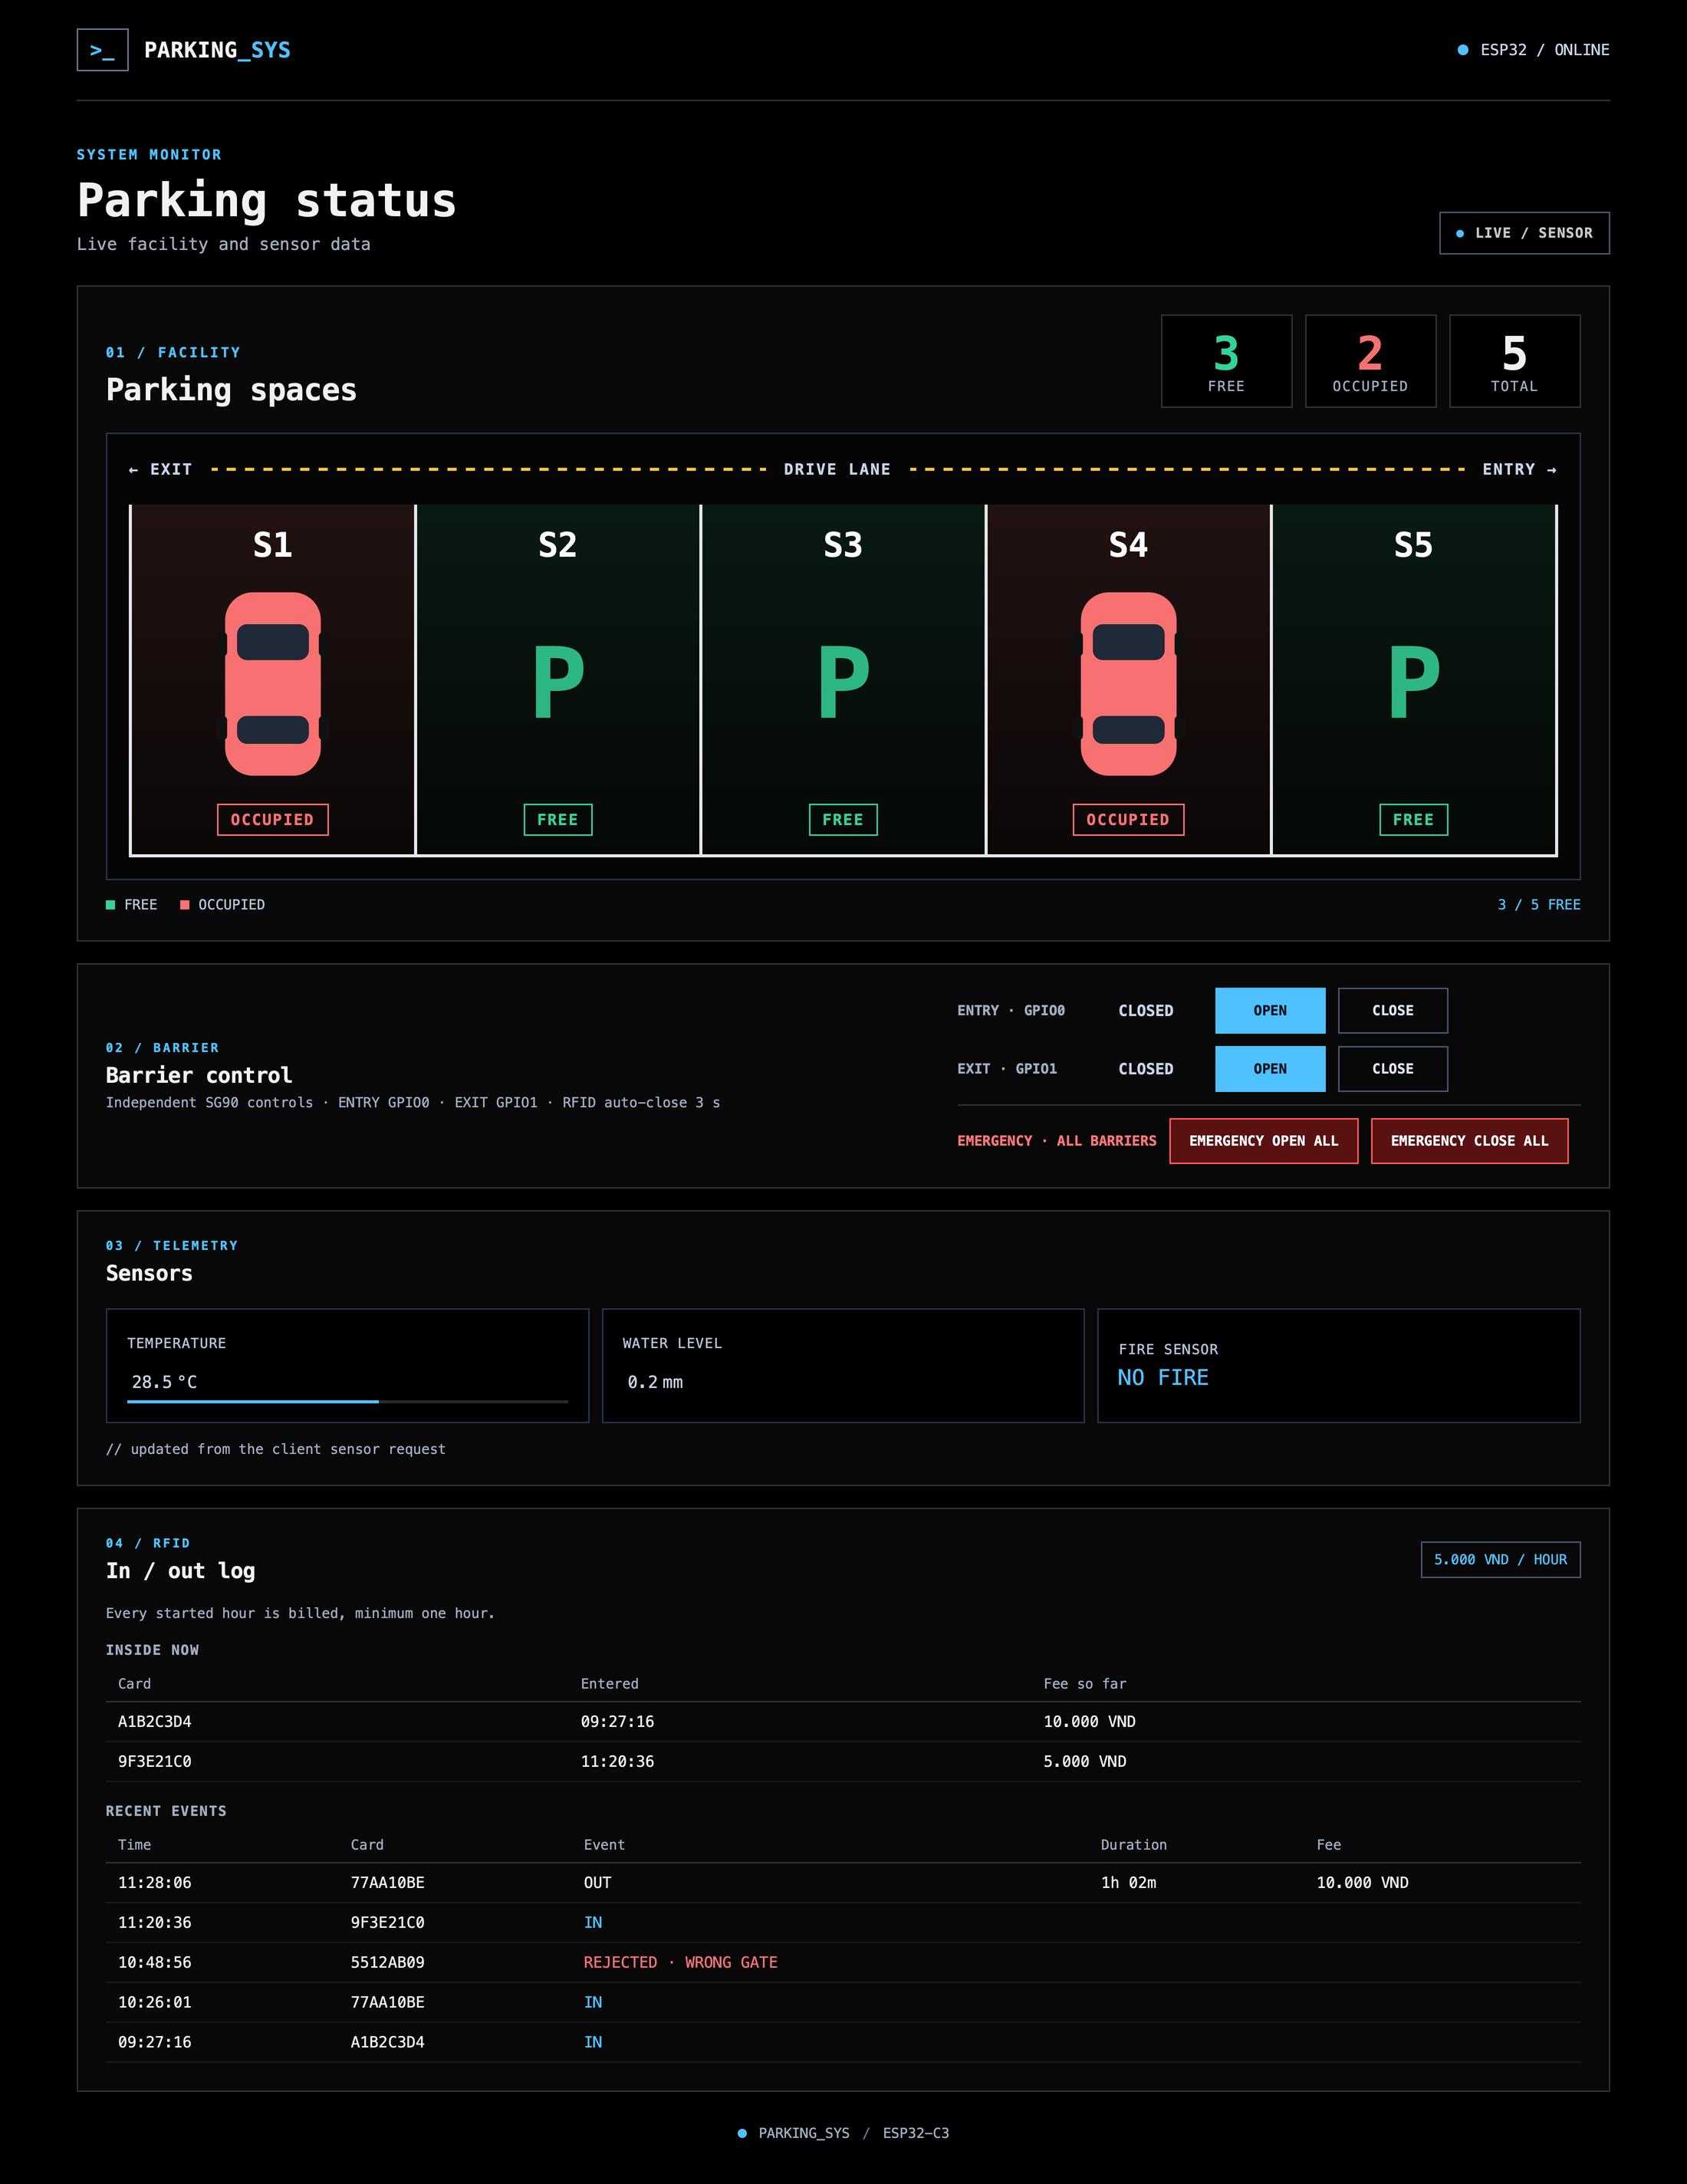
\includegraphics[width=0.86\linewidth]{dashboard.png}
\caption{Trang web giám sát tại \code{http://parking.local} (dữ liệu mẫu)}\label{fig:dashboard}
\end{figure}

\subsection{Các màn hình TFT}
\newcommand{\tftframe}[1]{%
\begin{tikzpicture}[x=0.0146cm,y=-0.0146cm,font=\tiny]
\fill[black] (0,0) rectangle (240,240);
#1
\draw[gray] (0,0) rectangle (240,240);
\end{tikzpicture}}
\newcommand{\tfttop}{%
\fill[cyan!70!blue] (0,0) rectangle (240,4);
\node[white,anchor=west,font=\tiny\bfseries] at (10,18) {PARKSENSE};
\node[gray!60,anchor=west,font=\fontsize{4}{4}\selectfont] at (10,44) {FREE SPACES};
\node[white,anchor=west,font=\scriptsize\bfseries] at (10,64) {3/5};
\fill[gray!25!black] (8,87) rectangle (68,127);
\fill[gray!25!black] (75,87) rectangle (135,127);
\node[white,anchor=west,font=\fontsize{4}{4}\selectfont] at (12,110) {28.0};
\node[white,anchor=west,font=\fontsize{4}{4}\selectfont] at (79,110) {0.2};
\fill[pink!50] (144,40) rectangle (240,136);
\foreach \i/\c in {0/red,1/green,2/green,3/red,4/green}{
  \fill[gray!25!black] (8+\i*46,147) rectangle (51+\i*46,190);
  \fill[\c] (8+\i*46,147) rectangle (11+\i*46,190);}
\fill[gray!25!black] (0,194) rectangle (240,240);}
\begin{figure}[H]
\centering
\setlength{\tabcolsep}{3pt}\begin{tabular}{cccc}
\tftframe{\tfttop
  \fill[orange!80] (90,205) rectangle (130,235);}
&
\tftframe{\tfttop
  \node[white,anchor=west,font=\fontsize{4}{4}\selectfont] at (8,201) {ID A1B2C3D4};
  \node[white,anchor=west,font=\fontsize{5}{5}\selectfont] at (8,226) {1H 01M};
  \node[cyan,anchor=west,font=\scriptsize\bfseries] at (126,222) {10000};}
&
\tftframe{\tfttop
  \node[white,anchor=west,font=\fontsize{4}{4}\selectfont] at (8,200) {ID 5512AB09};
  \node[red,anchor=west,font=\fontsize{6}{6}\selectfont\bfseries] at (8,215) {WRONG GATE};
  \node[gray!60,anchor=west,font=\fontsize{3.5}{3.5}\selectfont] at (8,232) {ALREADY INSIDE - USE EXIT GATE};}
&
\tftframe{\fill[red] (0,0) rectangle (240,8); \fill[red] (0,232) rectangle (240,240);
  \fill[red!40!black] (16,16) rectangle (224,224);
  \node[white,font=\scriptsize\bfseries] at (120,40) {DANGER};
  \fill[red] (100,90) rectangle (140,150); \fill[orange] (108,105) rectangle (132,150); \fill[yellow] (114,125) rectangle (126,150);
  \node[yellow,font=\fontsize{5}{5}\selectfont\bfseries] at (120,182) {FIRE DETECTED};
  \node[white,font=\fontsize{5}{5}\selectfont\bfseries] at (120,208) {EVACUATE NOW};}
\\[2pt]
\small (a) Bình thường & \small (b) Hóa đơn khi ra & \small (c) Quẹt sai cổng & \small (d) Có cháy \\
\end{tabular}
\caption{Bốn trạng thái màn hình TFT $240\times240$ (mô phỏng bố cục theo mã nguồn \file{lcd\_display.c})}\label{fig:tft}
\end{figure}
Trên màn hình bình thường: hàng trên là số chỗ trống, hai ô nhiệt độ và mực nước,
ảnh động $96\times96$ ở góc phải, hàng giữa là 5 ô S1–S5 với vạch xanh (trống)/đỏ (có
xe), vùng chân dùng cho ảnh động nhỏ, hóa đơn hoặc thông báo.

\subsection{Kịch bản demo}
\begin{enumerate}
\item Bật RFID Client, máy chủ, Sensor Client; mở \code{http://parking.local} trên điện thoại.
\item Đặt xe mô hình vào ô S2: ô S2 trên TFT chuyển đỏ ngay, trên web hiện hình xe trong $\le$ 1\,s.
\item Quẹt thẻ ở cổng vào: thanh chắn vào mở rồi tự đóng sau 3\,s; web có dòng \code{IN}.
\item Quẹt lại thẻ đó ở cổng vào: màn hình báo \code{WRONG GATE – ALREADY INSIDE - USE EXIT GATE}.
\item Quẹt thẻ ở cổng ra: hóa đơn hiện trên TFT, thanh chắn ra mở; web có dòng \code{OUT} kèm phí.
\item Đưa bật lửa gần cảm biến lửa: còi kêu, màn hình DANGER, hai thanh chắn mở và không đóng được từ web.
\item Tắt lửa: còi tắt, thanh chắn đóng, màn hình trở lại bình thường.
\end{enumerate}
